%%%%%%%%%%%%%%%%%%%%%%%%%%%%%%%%%%%%%%%%%%%%%%%%%%%%%%%%%%%%%%%%%%%%%%%%%%%%%%%
% Definici�n del tipo de documento.                                           %
% Posibles tipos de papel: a4paper, letterpaper, legalpapper                  %
% Posibles tama�os de letra: 10pt, 11pt, 12pt                                 %
% Posibles clases de documentos: article, report, book, slides                %
%%%%%%%%%%%%%%%%%%%%%%%%%%%%%%%%%%%%%%%%%%%%%%%%%%%%%%%%%%%%%%%%%%%%%%%%%%%%%%%
\documentclass[10pt, spanish, a4paper]{article}

%%%%%%%%%%%%%%%%%%%%%%%%%%%%%%%%%%%%%%%%%%%%%%%%%%%%%%%%%%%%%%%%%%%%%%%%%%%%%%%
% Los paquetes permiten ampliar las capacidades de LaTeX.                     %
%%%%%%%%%%%%%%%%%%%%%%%%%%%%%%%%%%%%%%%%%%%%%%%%%%%%%%%%%%%%%%%%%%%%%%%%%%%%%%%
\usepackage[spanish]{babel}     % Paquete para definir el idioma usado.
\usepackage[latin1]{inputenc}   % Define la codificaci�n de caracteres 
                                % (latin1 es ISO 8859-1)
%\usepackage[T1]{fontenc}        % Agrega caracteres extendidos al font
\usepackage{t1enc}
\usepackage{palatino}           % Cambia el font por omision a Palatino
\usepackage{graphicx}           % Paquete para inclusi�n de gr�ficos.
%%%%%%%%%%%%%%%%%%%%%%%%%%%%%%%%%%%%%%%%%%%%%%%%%%%%%%%%%%%%%%%%%%%%%%%%%%%%%%%

% Modifico los margenes para tener m�s espacio por linea
\oddsidemargin 0.0in    % margen derecho
\evensidemargin 1.0in   % margen izquierdo
\textwidth 6.0in        % ancho del texto

% T��tulo principal del documento.
\title{\textbf{The Speaker (3era Entrega)}}

% Informaci�n sobre los autores.
\author{    
            Juan Manuel Barrenche, \textit{Padr�n Nro. 86.152}                 \\
            \texttt{ snipperme@gmail.com }                                     \\
            Mart��n Fern�ndez, \textit{Padr�n Nro. 88.171}                      \\
            \texttt{ tinchof@gmail.com }                                       \\
            Marcos J. Medrano, \textit{Padr�n Nro. 86.729}                     \\
            \texttt{ marcosmedrano0@gmail.com }                                \\
            Federico Valido, \textit{Padr�n Nro. 82.490}                       \\
            \texttt{ fvalido@gmail.com }                                       \\ 
                                                                               \\
            \normalsize{Grupo Nro. 11 (YES)}                                   \\
            \normalsize{Ayudante: Renzo Navas}                         	       \\
            \normalsize{1er. Cuatrimestre de 2009}                             \\
            \normalsize{75.06 Organizaci�n de Datos - Titular: Arturo Servetto}\\
            \normalsize{Facultad de Ingenier�a, Universidad de Buenos Aires}   \\
       }
\date{Domingo 24 de Mayo de 2009}


% Comienzo del documento
\begin{document}

\maketitle                % Inserta el t�tulo.
\thispagestyle{empty}     % Quita el n�mero en la primer p�gina.

% Resumen que aparece en la primera p�gina (antes de la tabla de contenidos)
\begin{abstract}
Breve descripci�n de la arquitectura a utilizar para la 3era entrega del trabajo pr�ctico del curso de \textit{75.06 Organizaci�n de Datos} de la c�tedra Servetto.\\
Se detallan las clases e interfaces principales y su interacci�n, pero no se hace referencia a la arquitectura 
utilizada en las entregas anteriores ya que el punto de contacto con la nueva funcionalidad es m�nimo.
Este documento ha sido desarrollado en \LaTeX.
\end{abstract}

\newpage

\section{The Big Picture}

La idea principal es implementar los compresores como \textbf{Serializadores}. En nuestra arquitectura actual, los 
serializadores son utilizados en todos los manejadores de archivos (VLFM, StraightFM,...) para hidratar y deshidratar
objetos. \\
Implementar los compresores de esta manera tiene la ventaja de no tener que modificar nuestra arquitectura 
actual, que actualmente est� funcionando correctamente. Simplemente se reemplazan serializadores actuales por los
nuevos serializadores que ser�n capaces de comprimir, en nuestro caso, los Documentos.

\begin{figure}[!htp]
\centering
\makebox[\textwidth]{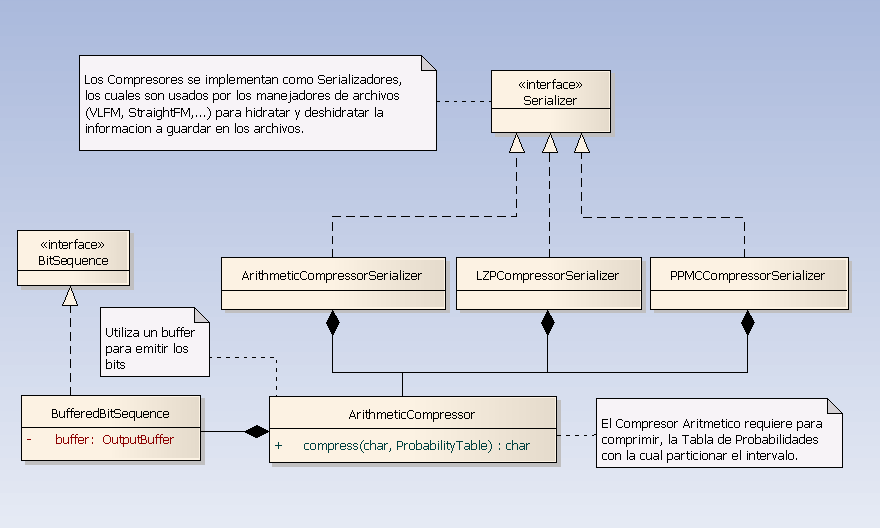
\includegraphics[scale=0.5,natwidth=20pt,natheight=10pt]{img/general.png}}
	\caption{Diagrama de clases general de la arquitectura propuesta}
\end{figure}

\section{Compresor Aritm�tico}
La clase \textit{ArithmeticCompressor} es el compresor aritm�tico \textit{per se}. Encargado de determinar que bits 
deben ser emitidos de acuerdo a la tabla de probabilidades que se le entrega y al caracter que se le indica que 
corresponde ser emitido. Dado que nuestros buffers trabajan de a bytes el compresor delega en un wrapper de dicho 
buffer que permite ingresar la informaci�n de a un bit por vez (y que luego emite de a bytes compltos). Luego, el 
compresor va iterando sobre los caracteres de la tabla (Que, si bien se muestran como char, esta clase es un wrapper de 
la clase Character de Java, ver mas adelante) y calcula los pisos y techos para cada caracter hasta que encuentre que 
el caracter a emitir \textit{matchea} con el caracter iterado. Luego de verificar si hay Overflow o Underflow, y emitir 
lo que corresponda, actualiza su piso y techo para estar listo para un nuevo caracter a emitir.
\newpage
El proceso de descompresi�n es el proceso inverso, en base a la tabla de probabilidades va armando los pisos y techos 
del caracter actual hasta que encuentra que la informaci�n de su buffer se encuentra dentro de dicho rango. Actualiza 
Overflow y Underflow, si corresponde, y devuelve el caracter correspondiente al nuevo rango para que el que el usuario 
del compresor pueda actualizar contextos y dem�s tareas.

\subsection{La clase Char}
La clase \textit{Char} permite tener valores fuera de los reales en un texto, es decir, el caracter \textbf{EOF}, y el 
caracter de \textbf{Escape}, que utiliza PPMC. Este �ltimo caracter tiene la particularidad que matchea con cualquier 
caracter, de manera que, en PPMC, estando en un contexto en el que no existe el caracter buscado, cuando el 
\textit{ArithmeticCompressor} verifica si el caracter matchea siempre va a encontrar que el de Escape si matchea. Es 
por esto que el compresor debe devolver el caracter de la tabla que encontr� matcheo con el recibido para que el PPMC 
pueda actuar seg�n corresponda.

\section{PPMC}

En cuanto a la arquitectura para el PPMC no hay mucho que decir, simplemente la clase PPMC se encarga de mantener las 
frecuencia de ocurrencia de los caracteres de cada contexto, las cuales se encuentran encadenadas de acuerdo a 
subniveles para facilitar la b�squeda, y de recordar cual es el contexto actual para pedirle al compresor aritm�tico 
que emita con dicha tabla de probabilidades. Cuando llama al aritm�tico arma la tabla de probabilidades excluyendo, si 
corresponde, los caracteres que otro contexto ya verific� en su tabla de frecuencias.

\begin{figure}[!htp]
\centering
\makebox[\textwidth]{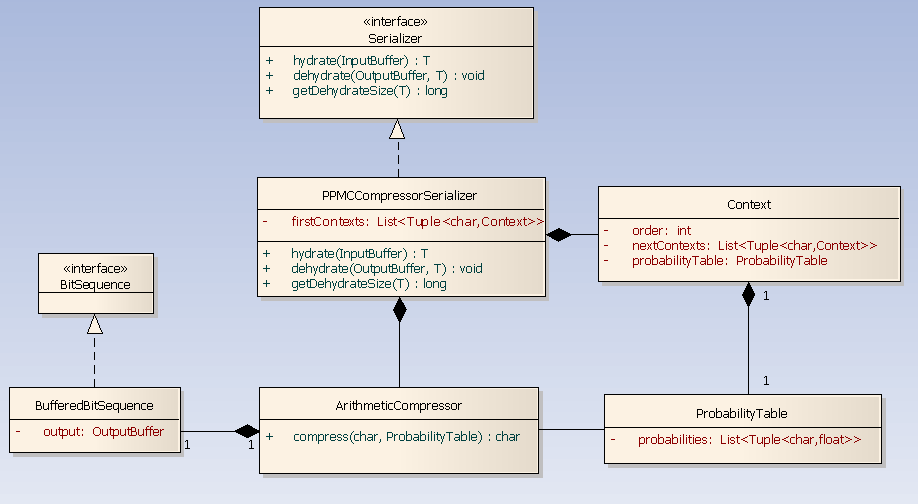
\includegraphics[scale=0.5,natwidth=20pt,natheight=10pt]{img/ppmc.png}}
\caption{Diagrama de clases de la arquitectura para PPMC}
\end{figure}

\end{document}
